\chapter{Implementacja}
\section{Wprowadzenie}
Celem tego rozdziału jest szczegółowy opis podejścia do realizacji projektu BBS, a mianowicie wyjaśnienie podstawowych pojęć, analiza architektury oraz algorytmów stosowanych do przetwarzania danych.

Chciałbym zacząć od tego, czym właściwie jest BBS. Zgodnie z definicją projekt jest w rzeczywistości procesorem języka \cite{compilers}, a konkretnie tłumaczem według następujących cech, które wynikają bezpośrednio z wymagań opisanych w rozdziale 2 \ref{design}:
\begin{itemize}
    \item Oprogramowanie analizuje kod wejściowy, napisany w specjalnie opracowanym na potrzeby projektu języku
    \item Oprogramowanie powinno wykrywać i raportować możliwe błędy logiczne lub składniowe w pliku wejściowym
    \item Zamiast tłumaczyć plik wejściowy na inny język programowania, program powinien wykonać polecenia opisane w pliku wejściowym
\end{itemize}

Dodatkowo oprogramowanie to zawiera również preprocesor. Dzieje się tak, aby plik wejściowy mógł zostać podzielony na wiele części, co umożliwi działanie mechanizmu budowania podprojektu.

\section{Gramatyka języka}

W tej sekcji wprowadzimy notację -- „gramatykę bezkontekstową” lub dla zwięzłości „gramatykę” -- która jest używana do definiowania składni języka. Gramatyka będzie używana w tej dokumentacji do organizowania interfejsu kompilatora. Gramatyka w naturalny sposób opisuje hierarchiczną strukturę większości struktur językowych \cite{compilers}. Używając zmiennej \texttt{expr} do oznaczenia wyrażenia i zmiennej \texttt{stmt} do oznaczenia instrukcji, tę regułę strukturyzacji można wyrazić jako :

\begin{lstlisting}[label=list:example_grammar,caption=Przykładowy opis gramatyki,basicstyle=\footnotesize\ttfamily]
<stmt> ::= "if" "(" <expr> ")" <stmt> "else" <stmt>
\end{lstlisting}

w której ''::='' można odczytać jako „może mieć formę”. Taka zasada nazywa się „produkcją”. Produkty posiadają takie elementy leksykalne, jak słowo kluczowe \texttt{if} i nawias, nazywane są „terminalami”. Zmienne takie jak \texttt{expr} i \texttt{stmt} reprezentują sekwencje terminali i nazywane są „nieterminalami”.

Gramatyka bezkontekstowa składa się z czterech elementów:
\begin{itemize}
    \item Zestaw znaków końcowych, czasami nazywany „leksemami”. Terminale to podstawowe symbole języka zdefiniowane przez gramatykę.
    \item Zbiór nieterminali, czasami nazywany „zmiennymi składniowymi”. Każdy nieterminal reprezentuje zestaw ciągów końcowych ciągów końcowych lub innych nieterminali
    \item Zbiór produkcji, gdzie każda produkcja składa się z nieterminala, zwanego głową lub lewą stroną produkcji, strzałki oraz sekwencji terminali i nieterminali, zwanej treścią lub prawą stroną produkcji.
    \item Oznaczenie jednego z nieterminali jako symbolu początkowego.
\end{itemize}

W celu opisu gramatyki będziemy musieli się posługiwać notacją BNF, która jest jedną z najprostszych i najczęściej używanych. O niej dalej.

\subsection{Backus-Naur Form (BNF)}

Backus-Naur Form (BNF) to formalna notacja używana do opisywania składni języków programowania oraz innych formalnych struktur. BNF pozwala definiować reguły gramatyczne w sposób precyzyjny, umożliwiając zrozumienie i implementację języka. Jest ona powszechnie stosowana w tworzeniu kompilatorów, interpreterów oraz dokumentacji języków programowania.

BNF składa się z zestawu reguł, z których każda opisuje, w jaki sposób można skonstruować element języka. Reguły te są definiowane za pomocą produkcji w postaci:

\begin{verbatim}
<nazwa-symbolu> ::= <elementy-składniowe>
\end{verbatim}

Symbol \texttt{::=} oznacza „jest definiowane jako” i oddziela nazwę symbolu nieterminalnego (po lewej stronie) od jego definicji (po prawej stronie). Symbol nieterminalny jest konstrukcją, która wymaga dalszego rozwinięcia w postaci innych symboli terminalnych lub nieterminalnych.

\paragraph{Znaczenie używanych symboli w BNF:}
\begin{itemize}
    \item \textbf{Symbol \texttt{|}}: Służy do reprezentacji alternatywy, wskazując, że dowolny z podanych elementów może zostać wybrany. Na przykład:
    \begin{verbatim}
    <digit> ::= "0" | "1" | "2"
    \end{verbatim}
    Definiuje, że \texttt{<digit>} może być jednym z trzech symboli: \texttt{0}, \texttt{1}, lub \texttt{2}.
    
    \item \textbf{Kwadratowe nawiasy \texttt{[]}}: Oznaczają, że element wewnątrz nich jest opcjonalny. Jeśli nawiasy te są używane, to konstrukcja może, ale nie musi, zawierać podany element. Na przykład:
    \begin{verbatim}
    <optional-part> ::= "prefix" [<suffix>]
    \end{verbatim}
    Wskazuje, że \texttt{<optional-part>} może zawierać tylko \texttt{"prefix"} lub \texttt{"prefix"} wraz z \texttt{<suffix>}.
    
    \item \textbf{Klamry \texttt{\{\}}}: Oznaczają powtarzalność, wskazując, że element wewnątrz może wystąpić dowolną liczbę razy, w tym zero. Na przykład:
    \begin{verbatim}
    <list> ::= "item" {"," "item"}
    \end{verbatim}
    Wskazuje, że \texttt{<list>} może składać się z jednego elementu \texttt{"item"} lub wielu elementów oddzielonych przecinkami.
    
    \item \textbf{Trójkątne nawiasy \texttt{<>}}: Są używane do oznaczania symboli nieterminalnych, czyli tych, które wymagają dalszego rozwinięcia. Na przykład w produkcji:
    \begin{verbatim}
    <expr> ::= <term> | <term> "+" <term>
    \end{verbatim}
    Symbol \texttt{<expr>} jest nieterminalny, podczas gdy \texttt{term} wymaga definicji w kolejnej regule.
\end{itemize}

\subsection{Gramatyka języka BBS}

Główne wymagania stawiane językowi stosowanemu w projekcie BBS to prostota gramatyki, minimalna liczba słów kluczowych, typów danych i zmiennych wewnętrznych. W trakcie pracy powstał język o następującej gramatyce:

\begin{lstlisting}[label=list:grammar,caption=Gramatyka języka projektu BBS,basicstyle=\footnotesize\ttfamily]
<script> ::= <declarations> <statements>

<statements> ::= <statements> <statement> | <empty>
<statement> ::= "!prj" <string>
              | "!files" <array>
              | "!deps" <array>
              | "!cflags" <string>
              | "!pre" <string>
              | "!post" <string>
              | "!inc" <array>

<declarations> ::= <declarations> <declaration> | <empty>
<declaration> ::= "!let" <id> "=" <string>

<array> ::= "[" <elements> "]"
<elements> ::= <strings> ["," <variables>] | <variables> | <empty>
<strings> ::= <string> {"," <string>}
<variables> ::= <variable> {"," <variable>}

<string> ::= '"' <characters> <separators> <punctuators> '"'
<variable> ::= "$" <id>
<id> ::= <characters>

<characters> ::= <character> {<character>}
<character> ::= "A" | "B" | ... | "Z" | "a" | "b" | ... | "z"

<separators> ::= <separator> {<separator>}
<separator> ::= " "

<punctuators> ::= <punctuator> {<punctuator>}
<punctuator> ::= "/" | "-" | "_" | "." | ","
\end{lstlisting}

Jak widać z opisu gramatyki, język operuje na dwóch głównych typach danych: sekwencji symboli i tablicy (ciągów znaków). Każdy ciąg znaków może składać się z liter, separatorów i znaków interpunkcyjnych i musi być ujęty w cudzysłów. Z kolei tablica składa się z jednego lub większej liczby ciągów znaków oddzielonych przecinkami i ujętych w nawiasy kwadratowe.

Struktura tego języka składa się z deklaracji i wyrażeń.
\begin{itemize}
    \item Deklaracje służą do tworzenia nowych zmiennych.
    \item Wyrażenia opisują działania lub konfigurację projektu.
\end{itemize}

Deklaracje tworzące nowe zmienne muszą być napisane zgodnie z gramatyką, przy czym nazwa zmiennej może zawierać wyłącznie litery alfabetu łacińskiego, a jej wartość może być jedynie ciągiem znaków. Użycie zmiennej może znajdować się w środku ciągu znaków (co z kolei oznacza również możliwość użycia zmiennych wewnątrz tablic, ale tylko wtedy, gdy są one również ujęte w cudzysłów), w tym celu wystarczy użyć znak dolara obok nazwy zmiennej.

Wyrażenia z kolei opisują dokładnie, jakie słowa kluczowe są użyte w tej konfiguracji. Obecnie istnieje tylko 7 słów kluczowych, które muszą być obsługiwane przez język BBS:
\begin{itemize}
    \item \texttt{!prj} -- deklaracja projektu określająca jego nazwę będącą jednocześnie nazwą źródłowego pliku wykonywalnego
    \item \texttt{!pliki} -- udostępnia listę plików należących do projektu, które podczas budowy projektu zostaną skompilowane w jeden plik wykonywalny
    \item \texttt{!deps} -- lista podprojektów, od których zależy ten projekt; zostaną zbudowane przed głównym
    \item \texttt{!cflags} -- deklaracja parametrów kompilatora, które będą używane podczas kompilacji każdego pojedynczego pliku
    \item \texttt{!pre} -- polecenie, które zostanie wykonane przed etapem montażu tego projektu
    \item \texttt{!post} -- polecenie, które zostanie wykonane przed etapem montażu tego projektu
    \item \texttt{!inc} -- deklaracja listy folderów zawierających pliki nagłówkowe
\end{itemize}

Każde z tych słów kluczowych może zostać użyte tylko raz (tj. drugie użycie tego samego słowa kluczowego nie może łączyć danych). Warto również zauważyć, że w gramatyce języka nie bez powodu deklaracje mają pierwszeństwo przed wyrażeniami w pliku: jeśli deklaracja następuje po wyrażeniu korzystającym z zadeklarowanej zmiennej, to w tym przypadku program musi się zakończyć, wyświetlając komunikat o błędzie.

\section{Struktura interpretera}
Zgodnie ze standardową strukturą kompilatorów i interpreterów, oprogramowanie BBS implementuje część frontend (czyli tę, która przeprowadza analizę) prawie w całości, natomiast backend nie zajmuje się optymalizacją ani generowaniem kodu, ponieważ wykonuje on określone instrukcje na podstawie danych wejściowych (czyli proces syntezy de facto nie zachodzi) \cite{compilers}.

Jeśli patrzyć na dane oprogramowanie ze względu na ogólnie przyjęte fazy kompilacji (które odpowiadają opisanym powyżej częściom standardowego kompilatora lub interpretera), to BBS realizuje prawie wszystkie fazy frontendu, z wyjątkiem generowania kodu pośredniego. Wynika to z niepraktyczności generowania kodu pośredniego bez znaczących opcji jego dalszego wykorzystania. Więc BBS zamiast tej fazy ma swoją, specjalną fazę -- fazę wypełniania wewnętrznej struktury opisującej projekt, który ma zostać zbudowany z BBS. Sama konstrukcja, a także procesy zachodzące w tej fazie zostaną szczegółowo opisane w dalszej części.

Podejście do implementacji backendu zasadniczo różni się od standardowego: nie jest wymagane dalsze tłumaczenie kodu na inny język, nie są realizowane fazy generowania kodu w innym języku. Zamiast tego backend na podstawie informacji o projekcie dostarczonych użytkownikowi wybiera określone polecenia do kontrolowania i budowania projektów.

Schemat fazowy BBS wygląda następująco:

\begin{figure}[h]
    \centering
    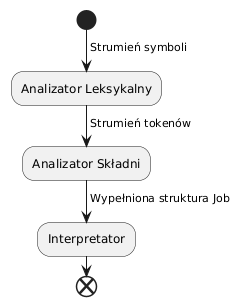
\includegraphics[width=0.4\textwidth]{Images/phases.png}
    \caption{Schemat fazowy projektu BBS}
\end{figure}

Następnie opis procesu implementacji programu zostanie podzielony na części, które również dzielą się na fazy. Ma to na celu proste opisanie procesów zachodzących w środku programu, a także zademonstrowanie danych wejściowych/wyjściowych.

\section{Analiza}
Jak opisano powyżej, dane wejściowe są analizowane w części frontendowej programu. Analizator dzieli dane wejściowe na części i narzuca im strukturę gramatyczną, która później posłuży do zbudowania projektu. Jeżeli parser stwierdzi, że dane wejściowe są niepoprawne składniowo lub semantycznie, informuje o tym użytkownika w najbardziej zrozumiały sposób. Dodatkowo analizator zbiera informacje w postaci tablicy symboli, co zostanie opisane w dalszej części.

\subsection{Analiza leksykalna}
Analiza leksykalna jest pierwszym etapem analizy danych wejściowych. Analizator leksykalny odczytuje strumień symboli i grupuje je w sensowną sekwencję zwaną leksemami, dla których analizator leksykalny generuje tzw. leksem składający się z typu pary -- odwołanie do tabeli symboli \cite{compilers}.

W projekcie BBS analizator leksykalny jest podzielony na dwie odrębne klasy, \texttt{Lexer} i \texttt{Scanner}, dla których zaimplementowana jest także klasa pomocnicza \texttt{Context}. Klasy te korzystają także z dodatkowych elementów, które zostaną opisane później (ale będą tu omawiane tylko te, które naprawdę zasługują na uwagę, np. nie będzie tu opisu klas wyjątków).

\subsubsection{Klasa Scanner}
Klasa \texttt{Scanner} jest osobną klasą, której delegowana jest rola odczytu plików. To właśnie w tej klasie hermetyzowane są wszelkie operacje sprawdzania istnienia, otwierania i odczytywania plików znak po znaku, a także omijania pustych linii czy komentarzy. Jego implementacja jest dość prosta, gdyż \texttt{Scanner} umożliwia odczytanie bieżącego znaku (funkcja \texttt{Get()}) i przejście do następnego (funkcja \texttt{Move()}). Z kolei operacja \texttt{Get()} opiera się na \texttt{std::optional} \cite{cpp_optional}, innowacji w C++17, która pozwala przechowywać wartość lub nic w bezpieczny i przejrzysty sposób. Klasa na wejściu otrzymuje nazwę pliku do odczytania, a na wyjściu zwraca przeczytany znak (odfiltrowując niepotrzebne), jeśli takie istnieją.

Na szczególną uwagę zasługuje metoda o nazwie \texttt{Skip()} (wywoływana wewnątrz metody \texttt{Move()}), która wykonuje operację pomijania komentarzy i pustych znaków w przypadku konieczności przeczytania kolejnej linii (czyli oznacza, że został znaleziony znak nowej linii). Ta metoda wygląda następująco:

\begin{lstlisting}[label=list:scanner,caption=Metoda Scanner::Skip(),basicstyle=\footnotesize\ttfamily]
void Scanner::Skip()
{
    // Read the next line if scanner finds a new line symbol, a comment or an empty line
    auto character = context_.GetCharacter();
    while(!character || character.value() == constants::kComment)
    {
        std::string line;
        std::getline(file_, line);
        if(file_.fail())
        {
            file_.close();
            return;
        }
    
        context_.Update(std::move(line));
        character = context_.GetCharacter();
    }
    
    // Check if the line still has anything to read
    if(!character || character.value() == '\0')
    {
        file_.close();
    }
}
\end{lstlisting}

Analizując ten kod, możemy stwierdzić, że \texttt{Scanner} najpierw odczytuje bieżący znak, który następnie przechodzi sprawdzenie istnienia (\texttt{std::optional} jest pusty, jeśli znak nie był czytany przez zamknięty plik, np.) lub równość określonego w gramatyce języka symbolu komentarza. Następnie, w przypadku pozytywnego wyniku kontroli (pusty znak lub komentarz), \texttt{Scanner} próbuje odczytać następną linię. Jeśli instrukcja się powiedzie, \texttt{Scanner} aktualizuje kontekst nową linią i zapamiętuje nowy znak jako bieżący, po czym powtarzane jest sprawdzenie istnienia znaku lub komentarza (ponieważ nowa linia może zawierać także komentarz). Przy wyjściu z pętli \texttt{Scanner} sprawdza, czy ostatnia linia została odczytana i jeśli odpowiedź jest pozytywna, plik jest zamykany.

\subsubsection{Klasa Context}
Między innymi moduł \texttt{lexer} zawiera ważną klasę pomocniczą \texttt{Context}, której wpływ na moduł jest dość znaczący. Klasa ta pojawiła się w procesie rozbudowy i rozwoju projektu BBS poprzez wyodrębnienie metod i pól z klasy \texttt{Scanner} w celu nie tylko spełnienia zasad SOLID \cite{solid}, ale także ułatwienia dostępu do informacji o bieżącej lokalizacji w pliku. Funkcjonalność ta służy w szczególności szczegółowemu informowaniu użytkownika o błędach składniowych lub semantycznych.

Klasa \texttt{Context} zawiera bieżącą linię przetwarzaną przez program, jej indeks w pliku oraz pozycję bieżącego znaku w linii. Wszystkie pola są chronione i dostępne pośrednio poprzez predefiniowany interfejs.

\subsubsection{Klasa Lexer}
Klasa \texttt{Lexer}, jak sama nazwa wskazuje, jest implementacją analizatora leksykalnego. Ta klasa jest najbardziej złożona ze wszystkich w module, a jej struktura jest modułowa, co ułatwia zmianę jej elementów w miarę zmiany wymagań lub gramatyki języka.

Główna klasa \texttt{Lexer} ma tylko metody manipulacji leksemami (\texttt{Get()} do odczytania bieżącego leksemu i \texttt{Next()} do żądania odczytania następnego leksemu), ponieważ praca z plikami została delegowana do klasy \texttt{Scanner}.

Proces kategoryzacji leksemów został delegowany do szeregu klas zwanych procedurami obsługi. Klasy te stanowią implementację wzorca projektowego „Łańcuch odpowiedzialności” \cite{cor}, który polega na przetwarzaniu określonych żądań przez dany obiekt i ich późniejszym przekazywaniu do kolejnych obiektów, w przypadku gdyby żądanie nie powiodło się. Ten wzorzec został użyty, aby wycofać użycie \texttt{switch-case}, aby umożliwić znacznie łatwiejsze (i jednolite) podłączanie nowych klas obsługi przy minimalnych zmianach w istniejącym kodzie (zgodnie z zasadami SOLID \cite{solid}). Klasy te posiadają następujący interfejs:

\begin{lstlisting}[label=list:handler,caption=Klasa Handler,basicstyle=\footnotesize\ttfamily]
/**
 * @brief A default Lexer input handler, an implementation of the CoR pattern
 * 
 */
class Handler
{
    using Token = parser::tokens::Token;
    
public:
    /**
     * @brief Process the input and return the token if possible
     * 
     * @param scanner - the source of characters to process
     * @return std::unique_ptr<Token> - a pointer to the token or nullptr 
     */
    virtual std::unique_ptr<Token> Process(Scanner& scanner) const;
    
    /**
     * @brief Set the next handler to be called to process the input
     * 
     * @param next - a pointer to the next handler to be called
     */
    void SetNext(std::unique_ptr<Handler> next);
    
protected:
    /**
     * @brief A pointer to the handler, next on the line to process the input
     * 
     */
    std::unique_ptr<Handler> next_;
};
\end{lstlisting}

Oznacza to, że każdy obiekt przetwarzający po utworzeniu otrzymuje łącze do następcy, do którego zostanie przekazane żądanie w przypadku niepowodzenia podczas jego realizacji. Jeśli żaden z programów obsługi nie był w stanie przetworzyć żądania, ostatni w łańcuchu tworzy wyjątek. Implementacja ta pozwoliła maksymalnie uprościć klasę \texttt{Lexer}, kod metody \texttt{Next()}, która wymusza na parserze odczytanie kolejnego tokena z pliku, dzięki wzorcowi „łańcuch odpowiedzialności” \cite{cor} został uproszczony do następującej postaci bez poświęcania stabilności i bezpieczeństwa programu:

\begin{lstlisting}[label=list:scanner,caption=Metoda Lexer::Next(),basicstyle=\footnotesize\ttfamily]
std::shared_ptr<Lexer::Token> Lexer::Next()
{
    token_ = std::move(handler_->Process(scanner_));
    return token_;
}
\end{lstlisting}

Klasa \texttt{Lexer} na wejściu otrzymuje nazwę pliku (która jest przekazywana do obiektu klasy Scanner i nie jest zapisywana bezpośrednio), na wyjściu \texttt{Lexer} zwraca aktualny leksem, a także umożliwia odczytanie nowy. W przypadku znalezienia nieznanych symboli, których nie przewidywała gramatyka języka, analizator tworzy odpowiedni wyjątek ze szczegółowym opisem położenia symbolu i przyczyną błędu.

Lista leksemów, które program może przetworzyć, odpowiada podanemu językowi i została opisana w sekcji „Gramatyk języka”.

\subsection{Analiza składni}

Po analizie leksykalnej lista leksemów wyodrębniona z plików wejściowych jest wysyłana do parsera. Praca parsera zazwyczaj polega na tworzeniu tzw drzewo składniowe, które jest pośrednią reprezentacją kodu wejściowego, odzwierciedlającą jego strukturę gramatyczną. Takie drzewo wygodnie zachowuje kolejność operacji i może wyglądać tak dla przykładowego wyrażenia $a = b + c$, gdzie $a$, $b$ i $c$ to identyfikatory dodane wcześniej do tablicy symboli:

\begin{figure}[h]
    \centering
    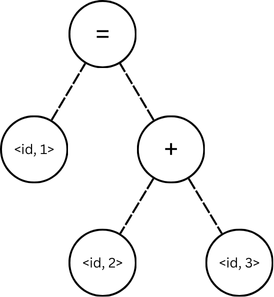
\includegraphics[width=0.4\textwidth]{Images/syntax_tree.png}
    \caption{Struktura gramatyczna przykładowego wyrażenia}
\end{figure}

Jak wspomniano w sekcji „Gramatyka języka”, opracowany język plików konfiguracyjnych projektu BBS jest dość prymitywny, co jest konsekwencją wymagań stawianych projektowi. Z tego powodu język nie obsługuje operacji arytmetycznych, łączenia ciągów znaków i zmiennych oraz nie zawiera żadnych innych typów danych niż typy „sekwencja znaków” i „tablica sekwencji znaków”. Biorąc pod uwagę wszystko, co napisano wcześniej, podjąłem decyzję o rezygnacji z implementacji parsera w taki sposób, aby możliwe było bezpośrednie utworzenie drzewa składniowego. Zamiast tego parser BBS, wykonując te same czynności, co wszystkie konwencjonalne parsery, natychmiast wykonuje funkcje zapisu danych projektu do pośredniej struktury danych.

Warto zaznaczyć, że parser ten stosuje podejście odgórne do analizy danych, czyli analizuje dane rozpoczynając od nieterminala początkowego i sprawdzając każdy symbol pod kątem zgodności z pochodnymi tego nieterminala. W przypadku BBS algorytm ten jest realizowany poprzez proste sprawdzenie danych wejściowych od lewej do prawej. Projektując, spośród innych algorytmów (np. oddolnych) wybrano ten algorytm ze względu na prostotę implementacji, a także ze względu na ogólną prostotę zaimplementowanego języka.

Pełna funkcjonalność parsera w projekcie BBS zaimplementowana jest w klasach \texttt{Parser}, \texttt{Mediator}, a także klasach wywodzących się z interfejsu \texttt{State}.

\subsubsection{Leksemy}

Danymi wejściowymi dla parsera są „leksemy” -- sklasyfikowane dane, które odbierane są na wyjściu leksera. Program BBS dla ogólnej prostoty, co jest jednym z głównych wymagań, używa języka z tylko dwoma typami danych i praktycznie bez instrukcji. Poniżej znajduje się lista wszystkich leksemów, które mogą zostać przetworzone przez program BBS. Wykonanie każdego z nich jest podobne i bardzo proste, dlatego nie będzie tutaj opisywane.

\begin{itemize}
	\item \texttt{Operator} -- „=” oraz „\$”
	\item \texttt{Punctuator} -- kropki, przecinki, nawiasy oraz wykrzykniki
	\item \texttt{Separator} -- spacje
	\item \texttt{Word} -- litery alphabetu lacińskiego
\end{itemize}

\subsubsection{Klasa Parser}

Najważniejszą klasą jest klasa \texttt{Parser}, która w rzeczywistości jest implementacją wzorca projektowego „State Machine” \cite{state}. Ten wzorzec projektowy służy do przeniesienia każdego stanu klasy do osobnej klasy z własną implementacją tych samych metod. Decyzja o zastosowaniu tego szablonu wynikała z faktu, że parser jest maszyną stanową w klasycznym sensie, gdyż rolą parsera jest sprawdzanie leksemu po leksemie, przy czym każdy kolejny leksem jest całkowicie syntaktycznie zależny od poprzedniego (tj. dany leksem może być oczekiwany lub nieoczekiwany, w zależności od leksemu, który był wcześniej przetwarzany przez parser).

Każdy stan parsera odpowiada oddzielnym nieterminalom zdefiniowanym w gramatyce języka użytego w projekcie. Interesująca jest implementacja każdego indywidualnego stanu, podczas gdy parser ma tylko jedną pełnoprawną metodę, która wywołuje metodę przetwarzania kolejnego znacznika bieżącego stanu i sprawdza istnienie tego stanu.


\begin{lstlisting}[label=list:parser,caption=Metoda Parser::Process(),basicstyle=\footnotesize\ttfamily]
scheduler::pipeline::Job Parser::Process()
{
    auto state = mediator_.GetState();
    while(state)
    {
        state->Process(lexer_);
    
        // Get the next state
        state = mediator_.GetState();
    }
    
    return mediator_.GetJob();
}
\end{lstlisting}

Każdy indywidualny stan implementuje wspólny dla wszystkich interfejs \texttt{State}, co zapewnia abstrakcję od szczegółów implementacji konkretnego stanu i znacznie upraszcza implementację samego parsera.

Ponadto ważnym elementem parsera jest także klasa \texttt{Mediator}, o czym będzie mowa później.

\subsubsection{Klasa Mediator}

Niezwykle ważną klasą jest klasa \texttt{Mediator}, która de facto jest implementacją znanego wzorca projektowego „Mediator”. Jego istotą jest uproszczenie połączeń pomiędzy klasami poprzez delegowanie metod komunikacji pomiędzy tymi klasami innej klasie zwanej „Mediatorem” \cite{mediator}.

W mojej implementacji parsera ta klasa jest potrzebna do uproszczenia zależności pomiędzy klasami \texttt{Parser}, każdą potomną interfejsów \texttt{State} i \texttt{Application}. Mediator ukrywa aktualny stan parsera, wskaźnik do obiektu struktury Job (o czym będzie mowa w następnej sekcji) oraz tablicę symboli. Wszystkie metody są w ten czy inny sposób getterami lub setterami, więc opisywanie ich implementacji nie jest tutaj szczególnie cenne.

\subsubsection{Klasy typów danych}

Jak już wspomniano, oprogramowanie to implementuje tylko dwa typy danych, a mianowicie „sekwencję znaków” i „tablicę sekwencji znaków”. Implementacja tych typów nie jest trudna i pod wieloma względami „tablica” opiera się na już istniejącej implementacji stanu „sekwencji znaków”, nie ma jednak pomiędzy nimi zależności hierarchicznych.

Każdy z tych typów implementuje interfejs \texttt{State}, co oznacza, że główną metodą, która nas interesuje w kontekście parsera jest \texttt{Process()}.

\begin{lstlisting}[label=list:string,caption=Metoda String::Process(),basicstyle=\footnotesize\ttfamily]
void String::Process(lexer::Lexer& lexer)
{
    // Skip separators in between the keyword and the
    auto token = State::SkipSeparators(lexer);

    // Expect the double quote mark at the start of the string
    Match(token.get(), ::parser::tokens::Punctuator::Type::kDoubleQuoteMark);
    
    // Add tokens one by one to the internal buffer
    while((token = lexer.Next()))
    {
        try
        {
            Match(token.get(), tokens::Punctuator::Type::kDoubleQuoteMark);
            return;
        }
        catch(const exceptions::UnexpectedTokenException&)
        {
            auto ptr = dynamic_cast<tokens::Operator*>(token.get());
            if(ptr && ptr->type == tokens::Operator::Type::kDollarSign)
            {
                Variable variable{mediator_};
                variable.Process(lexer);
    
                // Add variable's value to the result
                value_ += variable.GetValue();
    
                continue;
            }
    
            // Add the token to the whole value
            value_ += token->GetValue();
        }
    }
    
    throw exceptions::UnexpectedTokenException("");
}
\end{lstlisting}

Zacznijmy od przeanalizowania bardziej podstawowego typu „sekwencji znaków”. Jak widać z powyższego kodu, każda sekwencja zaczyna się i kończy podwójnymi cudzysłowami, więc kod najpierw sprawdza, czy bieżący leksem jest cudzysłowem. Następnie każdy kolejny leksem (dowolnego typu) jest dodawany do wartości sekwencji, aż program napotka znak cudzysłowu. Jeśli leksem końcowy nie jest cudzysłowem, program zakończy działanie, zgłaszając wyjątek.

Na szczególną uwagę zasługuje ciąg znaków sprawdzający obecność znaku dolara, który reprezentuje nazwę zmiennej, co zostanie omówione w dalszej części tego rozdziału. Przed dodaniem leksemu do pełnej wartości „ciągu znaków” parser sprawdza, czy nazwa zmiennej została odnaleziona. Jeżeli odpowiedź jest pozytywna, podejmowana jest próba zamiany nazwy zmiennej na jej wartość przy pomocy obiektu klasy \texttt{Variable}, który następnie jest dodawany do pełnej wartości „ciągu znaków”.


\begin{lstlisting}[label=list:array,caption=Metoda Array::Process(),basicstyle=\footnotesize\ttfamily]
void Array::Process(lexer::Lexer& lexer)
{
    // Skip separators in between the keyword and the
    auto token = SkipSeparators(lexer);

    // Expect the bracket at the start of the string
    Match(token.get(), tokens::Punctuator::Type::kLeftSquareBracket);

    // Process the tokens
    String string_handler{mediator_};
    do
    {
        // Get the next string
        string_handler.Process(lexer);
        value_.push_back(string_handler.GetValue());
        string_handler.Clear();

        // Get the terminator token
        token = SkipSeparators(lexer);

        // Try to match any punctuator
        try
        {
            Match(token.get(), tokens::Punctuator::Type::kRightSquareBracket);
            return;
        }
        catch(const exceptions::UnexpectedTokenException&)
        {
            Match(token.get(), tokens::Punctuator::Type::kComma);
        }
    } while(token);

    throw exceptions::UnexpectedEndOfFileException(lexer.GetContext());
}
\end{lstlisting}

Zamiast tego implementacja stanu \texttt{Array} jest bardziej złożona, ponieważ zamiast pojedynczego znaku kończącego, takiego jak cudzysłowy w ciągu znaków, tablica używa przecinków do oddzielania kolejnych sekwencji znaków, a także nawiasów kwadratowych aby zaznaczyć krawędzie tablicy. Zamiast tego w kodzie przetwarzającym ciągi znaków wykorzystano gotową klasę \texttt{String}, co znacznie upraszcza implementację tablic oraz poprawia jakość, stabilność i czystość kodu.

\subsubsection{Klasy słów kluczowych}

Implementacja każdego słowa kluczowego wymagała oddzielnych klas, ale w rzeczywistości wszystkie z nich są potomkami klas \texttt{String} lub \texttt{Array} (w zależności od cech gramatycznych konkretnego słowa). Podobnie jak omówione powyżej klasy typu bazowego, klasy każdego pojedynczego słowa posiadają własną implementację metody \texttt{Process()}, która służy do przetwarzania leksemów otrzymanych od obiektu klasy \texttt{Lexer}. Wszystkie słowa są opisane w sekcji „Gramatyka języka”.

Przykładem słowa kluczowego wywodzącego się z typu „sekwencja znaków” jest \texttt{cflags}, czyli słowo definiujące parametry kompilacji projektu. Jak widać z poniższego kodu, w metodzie \texttt{Process} odpowiedniej klasy najpierw wykonywana jest metoda klasy nadrzędnej, a następnie wynikowa wartość przekazywana jest do obiektu klasy \texttt{Job} poprzez odpowiednie wywołanie metody. Sam obiekt uzyskuje się poprzez wywołanie modułu pobierającego obiekt mediatora. Ostatnim krokiem jest przejście do stanu standardowego \texttt{Statement}, który rozpoczyna cykl przetwarzania każdej linii od nowa (zgodnie z architekturą odgórną parsera).

\begin{lstlisting}[label=list:cflags,caption=Metoda CFlags::Process(),basicstyle=\footnotesize\ttfamily]
void CFlags::Process(lexer::Lexer& lexer)
{
    String::Process(lexer);

    // Set the compilation flags
    auto& job = mediator_.BorrowJob();
    job.SetCompilationFlags(std::move(GetValue()));

    // Return to the Statement state
    mediator_.SetState(std::make_unique<Statement>(mediator_));
}
\end{lstlisting}
    
Na szczególną uwagę zasługuje klasa \texttt{Keyword}, która jest implementacją stanu parsera odpowiadającego nieterminalowi o tej samej nazwie. Jej celem jest przejście do prawidłowego stanu słowa kluczowego w celu jego obsługi przez program, metoda \texttt{Process()} tej klasy jest niczym innym jak implementacją wzorca projektowego „Metoda wytwórcza \cite{factory-method} , wzór generujący. Metoda ta ma konstrukcję \texttt{switch-case} i nie różni się niczym innym.

\begin{lstlisting}[label=list:keywords,caption=Metoda Keyword::Process(),basicstyle=\footnotesize\ttfamily]
void Keyword::Process(lexer::Lexer& lexer)
{
    // Check if the next token exists
    const auto token = lexer.Next();
    if(!token)
    {
        throw exceptions::UnexpectedEndOfFileException(lexer.GetContext());
    }

    // Process the correct keyword
    const auto& keyword = token->GetValue();
    if(keyword == "cflags")
    {
        mediator_.SetState(std::make_unique<keywords::CFlags>(mediator_));
        return;
    }
    else if(keyword == "deps")
    {
        mediator_.SetState(std::make_unique<keywords::Deps>(mediator_));
        return;
    }
    else if(keyword == "files")
    {
        mediator_.SetState(std::make_unique<keywords::Files>(mediator_));
        return;
    }
    else if(keyword == "prj")
    {
        mediator_.SetState(std::make_unique<keywords::Project>(mediator_));
        return;
    }
    else if(keyword == "pre")
    {
        mediator_.SetState(std::make_unique<keywords::Pre>(mediator_));
        return;
    }
    else if(keyword == "post")
    {
        mediator_.SetState(std::make_unique<keywords::Post>(mediator_));
        return;
    }
    else if(keyword == "let")
    {
        mediator_.SetState(std::make_unique<keywords::Let>(mediator_));
        return;
    }
    else if(keyword == "inc")
    {
        mediator_.SetState(std::make_unique<keywords::Inc>(mediator_));
        return;
    }
    
    throw exceptions::UnexpectedKeywordException(lexer.GetContext(), token->GetValue());
}
\end{lstlisting}

\subsubsection{Klasa Variable}

Jedną z najważniejszych klas stanu i filarem funkcji wykorzystania i przetwarzania zmiennych języka projektu jest klasa \texttt{Variable}. Klasa ta zajmuje się wyłącznie przetwarzaniem nazw zmiennych i na wyjściu zwraca wartość tej zmiennej, jeśli została ona wcześniej dodana do tablicy symboli.

Implementacja tej klasy nie jest zbyt trudna, nie jest podobna do żadnej innej metody pokrewnych klas i opiera się w dużej mierze na obiekcie Mediator, który sam ma tablicę symboli.

\begin{lstlisting}[label=list:variables,caption=Metoda Variable::Process(),basicstyle=\footnotesize\ttfamily]
void Variable::Process(lexer::Lexer& lexer)
{
    // Check if EOF is reached
    const auto token = lexer.Next();
    if(!token)
    {
        throw exceptions::UnexpectedEndOfFileException(lexer.GetContext());
    }

    // Check if the ID is a word
    auto ptr = dynamic_cast<tokens::Word*>(token.get());
    if(!ptr)
    {
        throw exceptions::UnexpectedTokenException(token->GetValue());
    }
    
    value_ = mediator_.GetVariableValue(token->GetValue());
}
\end{lstlisting}

Jak widać z implementacji głównej metody klasy powyżej, pierwszym etapem jej pracy jest pobranie i sprawdzenie aktualnego leksemu pod kątem poprawności (nazwa zmiennej może być tylko słowem, w odróżnieniu od typu „sekwencja znaków”, który może zaakceptować prawie wszystko). Po wszystkich niezbędnych sprawdzeniach metoda zwraca wartość zmiennej, jeśli taka istnieje.

\subsubsection{Klasa Statement}

Ta klasa jest nieterminalną implementacją o tej samej nazwie. Ta klasa jest wyłącznie odpowiedzialna za sprawdzanie obecności wykrzyknika na początku każdego słowa kluczowego i przejście do stanu „Słowo kluczowe”.

\subsubsection{Klasa State}

Klasa \texttt{State} stanowi interfejs dla wszystkich klas stanu parsera, dzięki czemu już na etapie parsowania osiągana jest poprawna i wydajna architektura projektu. Jednak dodatkowo klasa ta zawiera bez przesady najważniejsze metody dla wszystkich stanów, a mianowicie

\begin{itemize}
	\item SkipSeparators() -- odpowiada za pomijanie znaków oddzielających
	\item Match() -- sprawdzanie typu interpunkcji pod kątem równości z bieżącym leksemem
\end{itemize}

Implementacja metody SkipSeparators() polega na odebraniu kolejnych leksemów z obiektu klasy \texttt{Lexer} i próbie ich skonwertowania do typu \texttt{Separator}. Pierwszy leksem nieseparator opuszcza pętlę i kończy funkcję.

\begin{lstlisting}[label=list:separator_skip,caption=Metoda State::SkipSeparators(),basicstyle=\footnotesize\ttfamily]
std::shared_ptr<tokens::Token> State::SkipSeparators(lexer::Lexer& lexer)
{
    std::shared_ptr<tokens::Token> token;
    while((token = lexer.Next()))
    {
        // Token might be nullptr, handle this case
        if(!token)
        {
            throw std::runtime_error("State::SkipSeparators() was called with nullptr.");
        }
    
        if(!dynamic_cast<tokens::Separator*>(token.get()))
        {
            break;
        }
    }
    
    return token;
}
\end{lstlisting}

Z kolei metoda \texttt{Match()} działa podobnie jak poprzednia: jej zasada polega na konwersji wskaźnika na leksem na typ \texttt{Punctuator}, który następnie jest sprawdzany pod kątem identyczności z żądanym.

\begin{lstlisting}[label=list:match,caption=Metoda State::Match(),basicstyle=\footnotesize\ttfamily]
void State::Match(tokens::Token* token, tokens::Punctuator::Type value)
{
    if(!token)
    {
        throw exceptions::UnexpectedTokenException("EOF");
    }
    
    const auto ptr = dynamic_cast<tokens::Punctuator*>(token);
    if(!ptr || ptr->type != value)
    {
        throw exceptions::UnexpectedTokenException(std::move(token->GetValue()));
    }
}
\end{lstlisting}

\subsection{Analiza semantyczna}

Analizator semantyczny wykorzystuje drzewo składni i informacje zawarte w tablicy symboli, aby sprawdzić program źródłowy pod kątem zgodności semantycznej z definicją języka. Gromadzi również informacje o typie i przechowuje je w drzewie składni lub tabeli symboli do późniejszego wykorzystania podczas pośredniego generowania kodu.
Na przykład wiele zdefiniowanych języków programowania wymaga, aby indeks tablicy był liczbą całkowitą; kompilator powinien zgłosić błąd, jeśli do indeksowania tablicy użyto liczby zmiennoprzecinkowej.

Ponieważ program BBS nie musi generować żadnego kodu (tj. nie jest kompilatorem), co oznacza, że nie musi generować drzewa składniowego, nie zaimplementowano etapu analizy semantycznej. Decyzja ta ilustruje także fakt, że początkowy wymóg nałożył duże ograniczenie na liczbę typów danych wewnętrznych sprawdzanych przez usługę BBS, a także typów, które nie wymagają odpowiedniej konwersji czy adresowania tablic. Podsumowując, analiza semantyczna nie stała się częścią programu BBS.

\section{Synteza}
Synteza jest jednym z kluczowych etapów procesu kompilacji, zaraz po analizie (leksemicznej, składniowej i semantycznej). Jego celem jest przekształcenie pośredniej reprezentacji aplikacji w docelową formę kodu, którą można uruchomić na wybranej platformie. Proces ten obejmuje generowanie, optymalizację i uzupełnianie kodu obiektowego. Cały proces przedstawia poniższy diagram:

\begin{figure}[h]
    \centering
    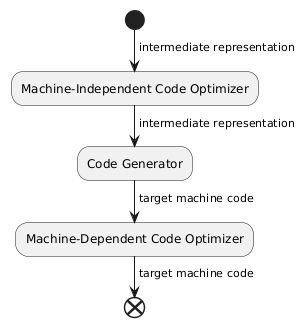
\includegraphics[width=0.4\textwidth]{Images/synthesis.png}
    \caption{Diagram procesu syntezy}
\end{figure}

Na początku syntezy kompilator pracuje z wewnętrzną reprezentacją kodu, na przykład:
\begin{itemize}
    \item Drzewo składniowe (AST -- Abstrakcyjne Drzewo Syntaktyczne),
    \item Kod trójadresowy lub inny format kodu pośredniego,
    \item Tablice symboli przechowujące informacje o zmiennych, funkcjach i ich właściwościach.
\end{itemize}

Jak wspomniano w poprzednich sekcjach, projekt BBS nie posiada kodu generującego drzewo składni w pełnym tego słowa znaczeniu (ani w ogóle żadnej pośredniej formy kodu). Wynika to z faktu, że w procesie syntezy BBS nie tłumaczy plików wejściowych bezpośrednio na kod maszynowy, lecz korzysta z gotowych rozwiązań (czyli gotowych kompilatorów, w większości przypadków jest to GNU GCC). I choć kompilacja plików wejściowych za pomocą BBS-a ma charakter pośredni, to i tak warto rozważyć ten proces na przykładzie gotowych rozwiązań, aby lepiej zrozumieć cel BBS-a i logikę jego działania.

\subsection{Generowanie kodu pośredniego}
Na wczesnym etapie syntezy generowany jest kod pośredni, będący abstrakcyjną reprezentacją logicznych operacji programu. Jego celem jest odejście od określonej architektury sprzętowej. Kod ten zawiera instrukcje o uproszczonej strukturze, które można łatwo przekształcić w kod maszynowy.

Kod pośredni jest często optymalizowany w celu poprawy wydajności programu. Proces ten może obejmować:
\begin{itemize}
    \item Eliminacja martwego kodu
    \item Optymalizacja pętli (rozmieszczenie pętli, niezmienny ruch kodu),
    \item Zmniejszenie liczby stosowanych rejestrów.
\end{itemize}

\subsection{Generowanie kodu maszynowego}
Na tym etapie kod pośredni jest konwertowany na kod maszynowy specyficzny dla wybranej architektury procesora. Generowanie kodu maszynowego obejmuje:

\begin{itemize}
    \item Przypisanie rejestrów procesora do zmiennych,
    \item Tłumaczenie instrukcji na zestaw operacji dostępnych na docelowym sprzęcie,
    \item Dodanie pewnych elementów, takich jak wektory przerwań lub wywołania systemowe.
\end{itemize}

\subsection{Łączenie i alokacja zasobów}
Synteza obejmuje również proces łączenia (t.zw. „linking”), w którym połączone pomiędzy sobą zostają różne moduły oprogramowania, w tym biblioteki dynamiczne i statyczne, a także rozwiązano odniesienia do symboli pomiędzy różnymi plikami. W wyniku tego procesu z wielu plików obiektowych powstaje jeden plik wykonywalny w jednej z poniżej wymienionych postaci:

\begin{itemize}
    \item Plik wykonywalny (np. ELF, PE),
    \item Kod odpowiedni do tłumaczenia (w przypadku tłumaczy),
    \item Kod bajtowy maszyny (np. dla maszyn wirtualnych takich jak JVM lub CLR).
\end{itemize}

\subsection{Opis procesu}

Jeśli chodzi o sam projekt BBS, proces syntezy w nim przebiega następująco: podczas analizy listy leksemów przez parser natychmiast wypełniana jest wewnętrzna struktura Job (jak już wspomniano, drzewo nie jest budowane bezpośrednio, ale Parser wykonuje akcje w oparciu o etapy przeglądania takiego drzewa), które następnie wykorzystywane są przez obiekt Pipeline, który z kolei wykonuje zgodnie z wewnętrznym planem stworzonym przez obiekt Scheduler. Obiekt klasy Pipeline odpowiada za kompilację i dalsze linkowanie każdego pliku, który jest powiązany z tym obiektem Job, w tym celu wykorzystywane są wywołania do wybranego przez użytkownika kompilatora (domyślnie jest to GNU GCC), któremu przekazywane są parametry kompilacji wzięte z tego samego obiektu klasy Job. Po pomyślnych wywołaniach podany katalog powinien zawierać plik wykonywalny w formacie odpowiadającym docelowemu systemowi operacyjnemu i architekturze procesora (ELF dla systemów UNIX-podobnych, PE dla Windows), który będzie miał taką samą nazwę jak nazwa podanego projektu przez użytkownika za pomocą słowa kluczowego \texttt{!prj} w pliku konfiguracyjnym.

\subsubsection{Kompilacja}
Jak wspomniano powyżej, BBS nie jest bezpośrednio odpowiedzialny za kompilację plików, skupiając się wyłącznie na zarządzaniu zależnościami pomiędzy plikami i projektami oraz skracając czas kompilacji, poprzez ignorowanie plików, które nie wymagają kompilacji (proces ten zostanie omówiony bardziej szczegółowo później).

Do kompilacji plików wejściowych określonych przez użytkownika w pliku konfiguracyjnym wykorzystywane są kompilatory istniejące w systemie (domyślnie jest to GNU GCC, który jest obecnie jedynym obsługiwanym kompilatorem). W celu prawidłowego wykorzystania różnych kompilatorów i uzyskania większej modułowości kodu utworzono warstwę abstrakcji składającą się z klas modułu \texttt{sys::tools::compilers}, potomków interfejsu Compiler, które realizują pomost pomiędzy BBS-em i kompilatorem, a także fabrykę, dzięki której można łatwo wybrać żądaną klasę kompilatora na podstawie parametrów przekazanych przez użytkownika poprzez plik konfiguracyjny.

Przed samą kompilacją BBS sprawdza, czy wskazane przez użytkownika pliki istnieją, czy są to pliki, a nie np. katalogi, co zapewnia poprawne działanie zastosowanych kompilatorów, obcinając bezwzględną większość błędów na etapie przygotowawczym: w przypadku wystąpienia jakichkolwiek problemów, BBS w trybie awaryjnym zakończy pracę, podświetlając szczegółowy opis każdego problemu wraz z lokalizacją błędu w pliku konfiguracyjnym.

Ponadto ważną częścią BBS jest optymalizacja procesu kompilacji na poziomie projektu. Oznacza to, że BBS powinien ujawnić pliki, które nie uległy zmianie od czasu ostatniej pełnej kompilacji określonego pakietu i uniemożliwić ich ponowną kompilację. Funkcjonalność ta zostanie opisana poniżej, gdyż dotyczy ona nie tylko etapu kompilacji, ale także linkowania, co wymusza umieszczenie jej opisu w osobnym rozdziale.

Jeżeli ani BBS, ani wybrany kompilator nie wykryli błędów i nie zakończyli poprawnie swojej pracy, pojawiają się tzw. pliki obiektowe, które zawierają tylko kod obecny w odpowiednim pliku wejściowym. Zamiast tego wszystkie odniesienia do funkcji zewnętrznych pozostają referencjami, które zostaną zastąpione właściwymi wywołaniami dopiero po prawidłowym zakończeniu procesu łączenia (więcej o tym później).

\subsubsection{Łączenie}
Podobnie jak w przypadku kompilacji, projekt BBS nie ma możliwości bezpośredniego łączenia plików obiektowych w jeden plik wykonywalny, rolę tę ponownie, z powodów opisanych wcześniej, powierzono gotowym rozwiązaniom. Domyślnie kompilator GNU GCC jest używany przez BBS zarówno jako kompilator, jak i linker.

Proces łączenia to ważny proces, którego celem jest utworzenie pojedynczego pliku wykonywalnego z wejściowych plików obiektowych w formacie specyficznym dla docelowego systemu operacyjnego i architektury procesora. Proces ten pobiera indywidualne funkcje każdego pojedynczego pliku wejściowego skompilowanego do kodu maszynowego i zmienia zewnętrzne, nierozwiązane wywołania na prawidłowe adresy wywołań funkcji lub zmienne zewnętrzne.

Ponieważ współczesne kompilatory mają możliwość łączenia gotowych plików obiektowych, do zaimplementowania procesu łączenia użyłem tej samej warstwy abstrakcji, co w przypadku procesu kompilacji.

\subsubsection{Optymalizacja procesu budowlanego}
Wracając do tematu optymalizacji budowy projektu, rozważmy następujący przypadek, który pozwoli nam pokazać wagę istnienia takiego rozwiązania jak BBS: istnieje pewien projekt A, który ma ponad 100 plików. Wybrany projekt został zbudowany, ale później tylko jeden plik został nieco zmodyfikowany, aby rozwiązać określony problem. W standardowym przypadku, korzystając z gotowych poleceń, najprawdopodobniej wszystkie pliki, nawet jeśli nie zostały zmienione, zostałyby przekompilowane, ponieważ wyszukiwanie tego samego wśród ponad 100 plików może być problematyczne i dawać rozwiązanie podatne na błędy. Sytuacja komplikuje się z każdym kolejnym plikiem, gdyż albo kompilacja będzie trwała zbyt długo, albo ze względu na ludzką naturę podczas kompilacji zostaną popełnione błędy. Takie sytuacje są niedopuszczalne, gdy w grę wchodzą ograniczenia narzucone przez Klienta.

Z tego powodu powstał projekt BBS, w którym natywne narzędzia kompilatora śledzą, które pliki uległy zmianie, dzięki czemu tylko te pliki zostaną ponownie skompilowane przy następnym wywołaniu BBS. Mechanizm ten działa w następujący sposób:

\begin{itemize}
    \item BBS odczytuje konfigurację projektu i ją analizuje
    \item Przed rozpoczęciem kompilacji BBS sprawdza każdy plik pod kątem zmian (tzn. czy czas modyfikacji pliku jest krótszy niż odpowiedni czas utworzenia pliku obiektowego)
    \item Jeżeli plik nie został zmieniony, przy pomocy kompilatora BBS otrzyma listę zależności dla tego pliku
    \item Każdą zależność sprawdzamy analogicznie jak plik główny z punktu 2.
    \item Po analizie plik, który nie został zmodyfikowany, jest ignorowany, BBS przechodzi do następnego pliku i rozpoczyna ten sam proces od kroku 1.
\end{itemize}

W rezultacie każdy niezmieniony plik jest odfiltrowywany, co w dużych projektach pozwala na znaczne skrócenie czasu kompilacji, przy jednoczesnym zmniejszeniu ryzyka problemów spowodowanych przez człowieka (co z kolei dodatkowo skraca czas testowania produktu i naprawiania nieistniejących problemów spowodowanych mieszaniem starych i nowych plików obiektowych).

Jako przykład należy przytoczyć implementację metody odbierającej listę plików, od których zależy dany plik, zapisaną z wykorzystaniem funkcji kompilatora GNU GCC.

\begin{lstlisting}[label=list:dependencies,caption=Implementacja metody GNUPlusPlus::GetDependencies(),basicstyle=\footnotesize\ttfamily]
std::vector<std::filesystem::path>
GNUPlusPlus::GetDependencies(const std::filesystem::path& file) const
{
	std::stringstream parameters;
	parameters << kFlags << " -MM " << file.string();

	// Add include directories
	for(auto& directory : kDirectories)
	{
		parameters << " -I " << directory.string();
	}

	SystemCommand command{kCompiler, parameters.str()};
	if(!command.Execute())
	{
		throw exceptions::CompilationErrorException(file);
	}

	// Clear the output from the unprintable symbols
	auto output = command.GetOutput();
	output.erase(
		std::remove_if(output.begin(), output.end(), [](auto x) { return std::iscntrl(x); }),
		output.end());

	// Split the output into a vector of files
	auto strings = Split(output, " ");
	std::vector<std::filesystem::path> dependencies;
	for(auto it = strings.begin() + 2; it != strings.end(); ++it)
	{
		dependencies.emplace_back(*it);
	}
	return dependencies;
}
\end{lstlisting}

Podane zestawienie pokazuje, jak obiekt klasy \texttt{Command} (co zostanie omówione później) wykonuje wcześniej przygotowane polecenie, którego celem jest uzyskanie listy zależności dla danego pliku. Proces ten przebiega następująco: najpierw tworzona jest lista parametrów, składająca się z pliku do analizy, listy folderów z nagłówkami oraz parametru kompilatora odpowiedzialnego za funkcję analizy zależności (w przypadku GNU GCC jest to \texttt{-MM} \cite{gcc} ). Następnie podejmowana jest próba wykonania polecenia, w przypadku niepowodzenia generowany jest wyjątek z informacją o przyczynie błędu i pliku, który spowodował ten błąd. Jeśli wykonanie polecenia powiedzie się, następnym krokiem będzie pobranie wyniku polecenia i podzielenie listy plików na poszczególne nazwy plików, aby ułatwić użycie funkcji \texttt{Split()} (nie będzie to omawiane w tym artykule, ponieważ jest to bardzo prosta funkcja).

\subsubsection{Klasa Job}

Jedną z klas podstawowych wymaganych do działania BBS jest klasa \texttt{Job}. Klasa ta nie jest implementacją żadnego wzorca i nie jest szczególnie wartościowa pod względem złożoności oprogramowania czy architektury, ale jest ważna, ponieważ zawiera wszystkie informacje o projekcie zebrane w procesie analizy. Składa się wyłącznie z metod pobierających i ustawiających, które bezpiecznie uzyskują dostęp do danych i przekazują je do docelowych klas lub metod.

Poniżej znajduje się lista danych, jakie można dodać do obiektu klasy \texttt{Job}:
\begin{itemize}
    \item Lista poleceń wykonywanych przed procesem budowy projektu
    \item Lista poleceń wykonywanych po zakończeniu procesu budowy projektu
    \item Parametry kompilatora
    \item Lista plików projektu
    \item Lista folderów, w których znajdują się tytuły
    \item Nazwa projektu i jego lokalizacja
    \item Lista zależności
\end{itemize}

Obiekt faktycznie jest właścicielem swoich danych, a aby uzyskać do nich dostęp, używane są stałe wskaźniki. Warto również zaznaczyć, że kopiowanie obiektu klasy \texttt{Job} jest zabronione (usunięto konstruktor i operator kopiowania). Odbywa się to w myśl założenia, że projektu nie należy kopiować, dane na jego temat powinny znajdować się w jednym miejscu dokładnie do momentu zakończenia budowy, po czym należy je usunąć ze względu na niepotrzebność.

\subsubsection{Klasy potomne interfejsu Command}

Jak wspomniano powyżej, kompilator używany do uruchamiania BBS jest oddzielnym programem wykonywanym za pomocą poleceń wydawanych systemowi. Oznacza to, że do wywołania kompilatora używane są narzędzia systemowe, do których dostęp istnieje za pośrednictwem wiersza poleceń lub wywołań systemowych. Żadna z tych metod nie jest jednak taka sama dla różnych systemów, co utrudnia spełnienie wymagań projektu BBS.

Język C++ pozwala na wykorzystanie specjalnego, ujednoliconego interfejsu do wykonywania poleceń systemowych w bardzo prosty i przejrzysty sposób. Takie rozwiązanie pozwala na abstrahowanie od różnic pomiędzy systemami docelowymi i skupienie się na realizacji ważniejszych komponentów programu. Dodatkowo zastosowanie wystandaryzowanego i przetestowanego kodu zwiększa niezawodność projektu, w którym jest on zastosowany, a także skraca czas jego realizacji.

Na samym początku wdrożenia wybrałem tę metodę ze względu na zalety wymienione w poprzednim akapicie, jednak bardzo szybko widoczne stały się ograniczenia, jakie narzuca zastosowanie tego podejścia: po wykonaniu polecenia funkcja \texttt{std::system} jest w stanie zwrócić tylko kod wykonania polecenia. Jest to wystarczające dla większości zadań postawionych przed BBS-em, ale dla jednej z głównych funkcji projektu ta wada jest krytyczna: chodzi o optymalizację kompilacji. Funkcja ta opiera się na możliwości współczesnych kompilatorów, przy założeniu poprawnych parametrów, zwrócenia listy plików, od których zależy dany plik. Ta funkcjonalność wykracza poza proste powiadamianie o stanie polecenia, dlatego \texttt{std::system} jest przestarzały.

Zamiast tego do realizacji tak ważnego procesu wybrano mechanizm potoków UNIX. Pozwala przekierować wyjście programu, a po jego zamknięciu uzyskać kod wykonawczy. Jednak to podejście ma wadę: nie jest przenośne, więc aby osiągnąć przenośność BBS na platformę Windows, należy oddzielić i uwzględnić implementacje klas hermetyzujących wykonywanie poleceń, w zależności od docelowego systemu operacyjnego. W tym celu stworzono wspólny interfejs Command, który jest implementowany przez klasy Command z dwóch różnych modułów: \texttt{nix} i \texttt{win} (obecnie nie zaimplementowane).

Oto implementacja klasy \texttt{Command} z modułu \texttt{nix}, która opiera się na mechanizmie potoków UNIX:

\begin{lstlisting}[label=list:command,caption=Metoda Command::Execute(),basicstyle=\footnotesize\ttfamily]
bool Command::Execute()
{
	auto pipe = popen(command_.c_str(), "r");
	if(!pipe)
	{
		return false;
	}

	std::array<char, 128> buffer;
	while(fgets(buffer.data(), static_cast<int>(buffer.size()), pipe) != nullptr)
	{
		output_ += buffer.data();
	}

	return pclose(pipe) == 0;
}
\end{lstlisting}

Jak widać, otwarcie potoku rozpoczyna się na podstawie polecenia przekazanego wcześniej konstruktorowi klasy \texttt{Command}, po czym należy sprawdzić, czy potok został utworzony. Następnie podejmowana jest próba odczytania danych wysyłanych poleceniem na standardowe wyjście, po czym funkcja \texttt{Execute} zwraca kod wykonania polecenia, który można odczytać po zamknięciu potoku. Dane wykonania polecenia zapisywane są do zmiennej wewnętrznej \texttt{output\_}, którą można odczytać za pomocą odpowiedniego modułu pobierającego.

Aby poprawnie użyć polecenia, które jest zaimplementowane wyłącznie dla właściwego systemu, należy w miejscu jego użycia dodać następujący blok kodu:

\begin{lstlisting}[label=list:include_command,caption=Podłączenie prawidłowej klasy Command,basicstyle=\footnotesize\ttfamily]
#ifdef __linux__
    #include "sys/nix/command.hpp"

    using Command = sys::nix::Command;
#endif
\end{lstlisting}

Kod ten zawiera plik napisany specjalnie dla systemu docelowego, a także tworzy alias dla klasy \texttt{Command} w celu wygodnego użycia.

\subsubsection{Klasy potomne interfejsu kompilatora}

Oprócz bezpośredniego wykonywania poleceń, w projekcie BBS ważna jest maksymalna abstrakcja od zewnętrznych bibliotek lub programów. Jest to konieczne, aby wyeliminować ewentualne ryzyko związane z aktualizacją interfejsów lub poleceń, które może pojawić się w przyszłości. Dlatego interakcja z kompilatorami wspieranymi przez projekt BBS odbywa się poprzez klasy potomne interfejsu \texttt{Compiler}. Wszystkie są implementacjami wzorca projektowego zwanego „Adapter” \cite{adapter}.

Główną zaletą szablonu „Adapter” jest jego prostota, a także możliwość hermetyzacji interakcji z interfejsami zewnętrznymi, dzięki czemu w przypadku ich zmiany projekt, który z nich korzysta, musi zostać zmieniony tylko w jednym miejscu. Takie podejście zwiększa bezpieczeństwo i niezawodność oprogramowania, a także skraca czas i koszty utrzymania produktu w przypadku zmiany zależności zewnętrznych.

Każda klasa implementująca interfejs Compiler musi mieć następującą strukturę: konieczne są tylko dwie główne metody, które zapewniają abstrakcję procesu kompilacji i uzyskują listę zależności.

\begin{lstlisting}[label=list:compiler,caption=Struktura interfejsu Compiler,basicstyle=\footnotesize\ttfamily]
struct Compiler
{
	/**
	 * @brief Compile the given file
	 * 
	 * @param file - the file to compile
	 * @param out - the file where to store the output
	 */
	virtual void Compile(const std::filesystem::path& file, const std::filesystem::path& out) = 0;

	/**
	 * @brief Get the dependencies of the file
	 * 
	 * @param file - the file to inspect
	 * @return std::vector<std::filesystem::path> - a vector of dependencies
	 */
	virtual std::vector<std::filesystem::path>
	GetDependencies(const std::filesystem::path& file) const = 0;
};
\end{lstlisting}

Ponieważ metoda \texttt{GetDependency()} została omówiona powyżej, tutaj opiszę szczegółowo drugą metodę, a mianowicie \texttt{Compile()} opartą na klasie potomnej \texttt{GNUPlusPlus}, która jest wymagana do pracy z Kompilator GNU GCC.

\begin{lstlisting}[label=list:gnu_compiler,caption=Implementacja metody GNUPlusPlus::Compile(),basicstyle=\footnotesize\ttfamily]
void GNUPlusPlus::Compile(const std::filesystem::path& file, const std::filesystem::path& out)
{
	std::stringstream parameters;
	parameters << kFlags << " -c " << file.string() << " -o " << out.string();

	// Add include directories
	for(auto& directory : kDirectories)
	{
		parameters << " -I " << directory.string();
	}

	SystemCommand command{kCompiler, parameters.str()};
	if(!command.Execute())
	{
		throw exceptions::CompilationErrorException(file);
	}
}
\end{lstlisting}

Metoda ta ma prostą strukturę: najpierw tworzony jest ciąg parametrów, które odpowiadają za nazwę plików wejściowych i wyjściowych uzyskanych poprzez parametry funkcji. Następnie każdy indywidualny katalog ze stałej \texttt{kDirectories} utworzony podczas konstruowania obiektu z parametrów konstruktora jest dodawany do parametrów jako katalog z nagłówkami (przy użyciu sekwencji parametrów z klawiszem \texttt{-I} na początku \cite{gcc}). Następnie wykonywana jest komenda, a w przypadku błędu metoda generuje wyjątek informujący o niemożności skompilowania tego pliku. W przypadku tego polecenia istotny jest parametr \texttt{-c}, wskazujący na konieczność utworzenia pliku obiektowego.

\subsubsection{Klasa Pipeline}

Klasa \texttt{Pipeline} służy do kontrolowania procesu budowy projektu od początku do końca. Klasa ta zawiera metody odpowiedzialne za każdą kolejną fazę budowania projektu, a mianowicie wykonanie poleceń przed kompilacją, weryfikację plików, kompilację, łączenie i wykonanie poleceń po kompilacji.

Wszystkie metody tej klasy wykorzystują wybrany kompilator do wykonania kompilacji i linkowania, a wykonanie poleceń polega na utworzeniu obiektów klasy \texttt{Command} odpowiadających systemowi operacyjnemu i wywołaniu jej metody \texttt{Execute} (opisanej powyżej).

Najciekawszą samodzielną funkcją tej klasy jest funkcja \texttt{IsCompiled()}, która sprawdza, czy plik został już skompilowany. Opiera się bezpośrednio na funkcjonalności kompilatora, który zwraca listę zależności dla danego pliku. Jest to jednak tylko część analizy, którą wykonuje metoda w celu ustalenia, czy dany plik wymaga kompilacji. Dodatkowo metoda analizuje czas utworzenia pliku obiektowego, czas ostatniej modyfikacji samego analizowanego pliku, a także każdy pojedynczy plik, od którego zależy pierwszy. Jeżeli którykolwiek z wymienionych plików został zmieniony po utworzeniu pliku obiektowego (o ile w ogóle istnieje), to plik nie jest uważany za skompilowany, co oznacza jego przebudowanie.

\begin{lstlisting}[label=list:is_compiled,caption=Implementacja metody Pipeline::IsCompiled(),basicstyle=\footnotesize\ttfamily]
bool Pipeline::IsCompiled(const std::filesystem::path& file,
						  const std::filesystem::path& folder) const
{
	// Check if the object file is built or created after the file was updated
	const auto obj = folder / file.filename().replace_extension(".o");
	if(!std::filesystem::exists(obj) ||
	   std::filesystem::last_write_time(file) > std::filesystem::last_write_time(obj))
	{
		return false;
	}

	const auto dependencies = compiler_->GetDependencies(file);
	for(const auto& dependency : dependencies)
	{
		if(std::filesystem::last_write_time(obj) < std::filesystem::last_write_time(dependency))
		{
			return false;
		}
	}

	return true;
}
\end{lstlisting}

\subsubsection{Klasa Executor}

Klasa \texttt{Executor} jest kluczowym komponentem organizującym i wykonującym sekwencję zadań reprezentowanych jako obiekty klasy \texttt{Pipeline}. Jego głównym celem jest uporządkowanie tych zadań poprzez przechowywanie ich w kolejce i przetwarzanie w kolejności, w jakiej zostały dodane. W tym celu używana jest standardowa struktura danych \texttt{std::queue}, która zapewnia dostęp do zadań według kolejności zgłoszeń.

Metoda \texttt{Add()} umożliwia dodanie do kolejki nowych obiektów Pipeline. Używa \texttt{std::move}, aby uniknąć niepotrzebnego kopiowania obiektu, co zwiększa wydajność. Dodanie do kolejki nie wykonuje samego zadania, a jedynie zapewnia, że jest ono gotowe do realizacji. Wykonanie zadania rozpoczyna się po wywołaniu metody \texttt{Run()}, która odpowiada za wykonanie wszystkich zadań w kolejce.

\begin{lstlisting}[label=list:executor,caption=Implementacja klasy Executor,basicstyle=\footnotesize\ttfamily]
void Executor::Add(pipeline::Pipeline pipeline)
{
	pipelines_.push(std::move(pipeline));
}

void Executor::Run()
{
	while(!pipelines_.empty())
	{
		// Run the pipeline
		const auto pipeline = std::move(pipelines_.front());
		pipeline.Run();

		// Pop the pipeline from the queue
		pipelines_.pop();
	}
}
\end{lstlisting}

\subsubsection{Klasa Application}

Główną klasą, która łączy wszystkie poprzednie, jest klasa \texttt{Application}. Ma to na celu konsekwentne wykonywanie faz analizy i syntezy, ale także zapewnienie prawidłowego działania całej aplikacji. Klasa ta zawiera metodę \texttt{Process()}, która odpowiada za utworzenie poprawnej kolejki zadań w obiekcie klasy \texttt{Executor}, a także za obsługę wszystkich wyjątków (w moim przypadku przetwarzanie odbywa się tak prosto, jak to możliwe, komunikat o wyjątku jest przesyłany na standardowe wyjście, a następnie aplikacja zostaje zakończona).

\begin{lstlisting}[label=list:application,caption=Implementacja metody Application::Process(),basicstyle=\footnotesize\ttfamily]
void Application::Process(std::filesystem::path path)
{
	parser::Parser parser{path / kBuildFile};
	try
	{
		auto job = parser.Process();
		job.SetProjectPath(path);

		// Process dependencies
		for(const auto& dependency : job.GetDependencies())
		{
			Process(path / dependency);
		}

		// Create a new pipeline to build the project
		scheduler::pipeline::Pipeline pipeline{std::move(job)};
		executor_.Add(std::move(pipeline));
	}
	catch(const std::exception& ex)
	{
		std::cout << ex.what() << std::endl;
		return;
	}
}
\end{lstlisting}